\section{Squark Production at One-Loop}
This section discusses the cross section for squark production at next-to-leading order $\sigma^{\mathrm{NLO}}$. To do so, the next section gives a justification why on-shell renormalization has been chosen in section \ref{sec:renMRSSM}. After that, the set up of the calculation, which has been performed by a \texttt{C++} program,  of the different contributions to $\sigma^{\mathrm{NLO}}$, is explained. This includes a remark on how the calculation was sped up. Finally the results of the computation are presented in the form of $K$-factors. These are then compared to the ones in the MSSM before the thesis closes with an discussion of the behavior of $\sigma^{\mathrm{NLO}}$ in the limit of large sgluon masses.

\subsection{The LSZ Theorem}\label{sec:LSZ}
The LSZ theorem\cite{Lehmann:1954rq} or LSZ reduction formula, named after  Harry Lehmann, Kurt Symanzik and Wolfhart Zimmermann, prescribes how to obtain the S-matrix element, i.e. a physical observable, from the time ordered correlation function of the respective field operators. The time ordered correlation function of fields in an interacting theory can be calculated perturbatively with the aid of the Gell-Mann and Low theorem and the Wick theorem. \\
Considering a physical process with kinematics $\vec{k}_1 \hdots \vec{k}_n \to \vec{p}_1 \hdots \vec{p}_m$ and taking for the sake of simplicity only one scalar field $\phi$ the Fourier transform of the time ordered product of a correlation function is related to the corresponding S-matrix element like\footnote{In this subsection the $\sim$ indicates that the poles on either side are the same provided that all momenta are close to their mass shell, i.e. $p_i^0 \to E_{\vec{p}_i}$ and $k_j^0 \to E_{\vec{k}_j}$.}
\begin{align}
\prod_{i=1}^n \int \mathrm{d}x_i\ \mathrm{e}^{ip_i x_i} \prod_{j=1}^m \int \mathrm{d}y_j\ \mathrm{e}^{ik_j y_j} \left\langle \Omega | \mathcal{T} \left[ \phi(x_1) \hdots \phi(x_n) \phi(y_1) \hdots \phi(y_m) \right] | \Omega\right\rangle \nonumber\\
\sim \prod_{i=1}^n \frac{i\sqrt{Z}}{p_i^2 - m^2 + i\epsilon} \prod_{j=1}^m \frac{i\sqrt{Z}}{k_j^2 - m^2 + i\epsilon} \left\langle \left.\left.\vec{p}_1 \hdots \vec{p}_n \right| S \right| \vec{k}_1 \hdots \vec{k}_m \right\rangle .\label{eq:LSZ}
\end{align}
Here $\mathcal{T}$ denotes the time ordering operator, $\left.| \Omega \right\rangle$ is the ground state of the interacting theory and $\sqrt{Z}$ is the residue of the single particle pole in the two-point function 
\begin{align}
\int \mathrm{d}x\ \mathrm{e}^{ip x} \left\langle \Omega | \mathcal{T} \left[ \phi(x) \phi(0) \right] | \Omega\right\rangle &= \frac{i}{p^2-m_0^2} + \frac{i}{p^2-m_0^2} \left(\frac{\Sigma(p^2)}{p^2-m_0^2}\right) + \frac{i}{p^2-m_0^2} \left(\frac{\Sigma(p^2)}{p^2-m_0^2}\right)^2 + \hdots\nonumber\\
&= \frac{i}{p^2 - m_0^2 - \Sigma(p^2)}.\label{eq:propagator}
\end{align}
\begin{figure}[!htbp]
\begin{center}
\begin{tikzpicture}[line width=2.0 pt, scale=1.3]
	\draw[fermionnoarrow](180:1)--(180:0.5);	
	\draw (0,0) circle (.5cm);
		\begin{scope}
	    	\clip (0,0) circle (.5cm);
	    	\foreach \x in {-1.0,-0.9,...,1.0}
        \draw[line width=1 pt] (\x,-.5) -- (\x+.6,.5);
	  	\end{scope}
	\draw[fermionnoarrow](0:0.5)--(0:1);
	\node at (1.3,0) {=};
	\draw[fermionnoarrow](0:1.6)--(0:2.6);
	\node at (2.9,0) {+};
    \draw[fermionnoarrow](0:3.2)--(0:3.7);	
	\draw (4.2,0) circle (.5cm);
	\node at (4.2,0) {1PI};
	\draw[fermionnoarrow](0:4.7)--(0:5.2);
	\node at (5.5,0) {+};	
	\draw[fermionnoarrow](0:5.8)--(0:6.3);	
	\draw (6.8,0) circle (.5cm);
	\node at (6.8,0) {1PI};
	\draw[fermionnoarrow](0:7.3)--(0:7.8);
	\draw (8.3,0) circle (.5cm);
	\node at (8.3,0) {1PI};
	\draw[fermionnoarrow](0:8.8)--(0:9.3);
	\node at (9.8,0) {+ $\hdots$};
\end{tikzpicture}
\caption{Diagrammatic figure of the two-point function of a scalar field: The propagator in an interaction theory can be calculated in a perturbation series in the coupling constant.}\label{fig:fullpropagator}
\end{center}
\end{figure}
The parameter $m_0$ is the tree-level mass and the quantity $-i \Sigma(p^2)$ denotes the sum of all one-particle-irreducible contributions to the particle's self-energy. From eq. \eqref{eq:propagator} one can read off the physical mass $m^2$ of the particle which is associated with the field $\phi$. It is determined as the value of $p^2$ where the propagator has a pole, i.e. 
\begin{align}
\left[ p^2 - m_0^2 - \Sigma(p^2)\right]_{p^2 = m^2} = 0
\end{align}
Close to the pole the denominator of eq. \eqref{eq:propagator} can by expanded like
\begin{align}
p^2 - m_0^2 - \Sigma(p^2) = (p^2 - m^2)\left( 1 - \frac{\partial \Sigma(p^2)}{\partial p^2} \right)_{p^2 = m^2} + \mathcal{O}((p^2 - m^2)^2).
\end{align}
The residue of the propagator can therefore be written as 
\begin{align}
Z = \left( 1 - \frac{\partial \Sigma(p^2)}{\partial p^2} \right)_{p^2 = m^2}^{-1}.
\end{align}
Now considers the full $(n+m)$-point function in scalar theory. One can decompose it into an amputated $(n+m)$-point function and ``full'' propagators like written in eq. \eqref{eq:propagator} and depicted in fig. \ref{fig:fullpropagator}.
\begin{figure}[!htbp]
\begin{center}
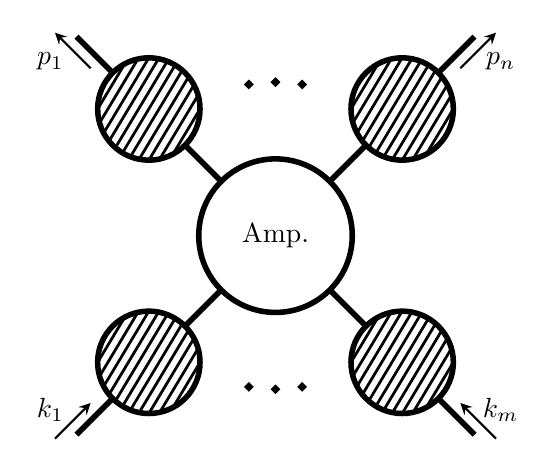
\begin{tikzpicture}[line width=2.0 pt, scale=1.3, arrow/.style={thick,->,shorten >=2pt,shorten <=2pt,>=stealth}]
	\draw (0,0) circle (.75);
	\node at (0,0) {Amp.};
	\draw (45:0.75)--(45:1.25);
	\draw (45:1.75) circle (.5);
		\begin{scope}[shift={(45:1.75)}]
	    	\clip (0,0) circle (.5cm);
	    	\foreach \x in {-1.0,-0.9,...,1.0}
        \draw[line width=1 pt] (\x,-.5) -- (\x+.6,.5);
	  	\end{scope}
	\draw (45:2.25)--(45:2.75);
	\draw[arrow] (1.768,1.597)--(2.192,2.021);
	\node at (2.2,1.7){$p_n$};

	\draw (135:0.75)--(135:1.25);
	\draw (135:1.75) circle (.5);
		\begin{scope}[shift={(135:1.75)}]
	    	\clip (0,0) circle (.5cm);
	    	\foreach \x in {-1.0,-0.9,...,1.0}
        \draw[line width=1 pt] (\x,-.5) -- (\x+.6,.5);
	  	\end{scope}
	\draw (135:2.25)--(135:2.75);
	\draw[arrow] (-1.768,1.597)--(-2.192,2.021);
	\node at (-2.2,1.7){$p_1$};	
	
	\draw (225:0.75)--(225:1.25);
	\draw (225:1.75) circle (.5);
		\begin{scope}[shift={(225:1.75)}]
	    	\clip (0,0) circle (.5cm);
	    	\foreach \x in {-1.0,-0.9,...,1.0}
        \draw[line width=1 pt] (\x,-.5) -- (\x+.6,.5);
	  	\end{scope}
	\draw (225:2.25)--(225:2.75);
	\draw[arrow] (-2.192,-2.021)--(-1.768,-1.597);
	\node at (-2.2,-1.7){$k_1$};	
	
	\draw (315:0.75)--(315:1.25);
	\draw (315:1.75) circle (.5);
		\begin{scope}[shift={(315:1.75)}]
	    	\clip (0,0) circle (.5cm);
	    	\foreach \x in {-1.0,-0.9,...,1.0}
        \draw[line width=1 pt] (\x,-.5) -- (\x+.6,.5);
	  	\end{scope}
	\draw (315:2.25)--(315:2.75);
	\draw[arrow] (2.192,-2.021)--(1.768,-1.597);
	\node at (2.2,-1.7){$k_m$};
	
	\draw[fill=black] (80:1.5) circle (.01);
	\draw[fill=black] (90:1.5) circle (.01);
	\draw[fill=black] (100:1.5) circle (.01);
	\draw[fill=black] (-80:1.5) circle (.01);
	\draw[fill=black] (-90:1.5) circle (.01);
	\draw[fill=black] (-100:1.5) circle (.01);
\end{tikzpicture}
\caption{Diagrammatic figure of a ``full'' $(n+m)$-point function. Apart from the ``full'' propagators there is the ``full'' amputated $(n+m)$-point function}
\end{center}
\end{figure}\\
Inserting the expression
\begin{align}
\frac{i}{p^2 - m_0^2 - \Sigma(p^2)} \sim \frac{i Z}{p^2 - m^2}
\end{align}
for the full propagators one notices the same singularity as in eq. \eqref{eq:LSZ}. Comparing the coefficients of these poles in eq. \eqref{eq:LSZ} one obtains
\begin{figure}[!htbp]
\begin{center}
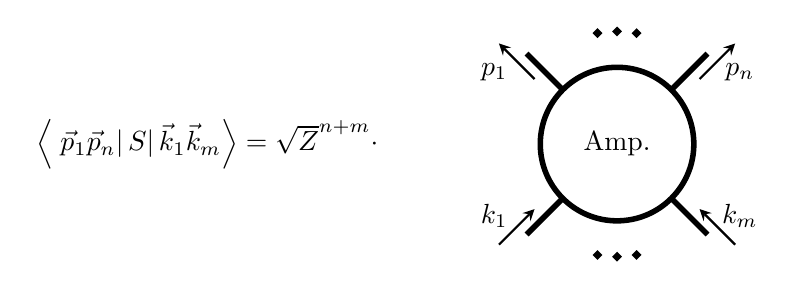
\begin{tikzpicture}[line width=2.0 pt, scale=1.3, arrow/.style={thick,->,shorten >=2pt,shorten <=2pt,>=stealth}]
	\node at (-4,0) {$\left\langle \left.\left.\vec{p}_1 \hdots \vec{p}_n \right| S \right| \vec{k}_1 \hdots \vec{k}_m \right\rangle =\sqrt{Z}^{n+m} \cdot$};
	\draw (0,0) circle (.75);
	\node at (0,0) {Amp.};

	\draw (45:0.75)--(45:1.25);
	\draw[arrow] (0.768,0.597)--(1.192,1.021);
	\node at (1.2,0.7){$p_n$};

	\draw (135:0.75)--(135:1.25);
	\draw[arrow] (-0.768,0.597)--(-1.192,1.021);
	\node at (-1.2,0.7){$p_1$};	
	
	\draw (225:0.75)--(225:1.25);
	\draw[arrow] (-1.192,-1.021)--(-0.768,-0.597);
	\node at (-1.2,-0.7){$k_1$};	
	
	\draw (315:0.75)--(315:1.25);
	\draw[arrow] (1.192,-1.021)--(0.768,-0.597);
	\node at (1.2,-0.7){$k_m$};
	
	\draw[fill=black] (80:1.1) circle (.01);
	\draw[fill=black] (90:1.1) circle (.01);
	\draw[fill=black] (100:1.1) circle (.01);
	\draw[fill=black] (-80:1.1) circle (.01);
	\draw[fill=black] (-90:1.1) circle (.01);
	\draw[fill=black] (-100:1.1) circle (.01);
\end{tikzpicture}
\end{center}
\end{figure}\\
Now it becomes clear, why the renormalization in the on-shell scheme
\begin{align}
\left.\frac{\partial \Sigma(p^2)}{\partial p^2}\right|_{p^2 = m^2} \stackrel{!}{=} 0
\end{align}
introduces no further modification, when turning from the Green function to the S-matrix-element because $Z = 1$ in on-shell renormalization. Furthermore the on-shell condition for the mass renormalization
\begin{align}
\Sigma(p^2)|_{p^2 = m^2} = 0
\end{align}
means that the physical mass equals the tree level mass.

\subsection{The Squark Production Cross Section at Next-to-Leading Order}
The squark production cross section at next-to-leading order is composed out of three contributions. These are the Born (tree-level) cross section, the virtual and the real corrections. 
\begin{align}
\sigma^{\mathrm{NLO}} = \sigma^{\mathrm{B}} + \sigma^{\mathrm{V}} + \sigma^{\mathrm{R}}\label{eq:BVR}
\end{align}
All three contributions have to be calculated with next-to-leading order parton density functions and $\alpha_s$. There are five mass scales: the squark mass $m_{\tilde{q}}$, the gluino mass $m_{\tilde{g}}$, the center of mass energy of the colliding protons $\sqrt{S}$, the top-quark mass which is fixed to $m_t = \unit[172]{GeV}$ and the mass of the pseudoscalar $m_{\sigma}$. The next section summaries how the calculation has been automated within a \texttt{C++} program.

\subsubsection{The Setup of the Calculation}
The setup of the calculation is summarized in fig. \ref{fig:CalcSetup}. Both the virtual and the Born matrix amplitude have been generated with the \texttt{Mathematica} package \texttt{FeynArts}. To this end a model file, generated by the \texttt{Mathematica} package \texttt{SARAH}, has been adjusted appropriately as described in section \ref{sec:ModelFileImplementation}. The matrix amplitudes have been processed further to $\sum|\mathcal{M}^{\mathrm{B}}|^2$ and $ \sum 2\Re (\mathcal{M}^{\mathrm{B}} \mathcal{M}^{\mathrm{1L}\ast})$ by the \texttt{Mathematica} package \texttt{FormCalc} before this output has then been converted to a \texttt{C++} readable code.
\begin{figure}[H]
\begin{center}
\begin{tikzpicture}
	\node [block4] at (-1,0) (Mathematica) {Mathematica notebook};
	\node [block1a] at (-1,-2.1) (notebookR) {soft/collinear limit: \newline \texttt{FeynArts} $\to \mathcal{M}^{\mathrm{R}}$ \newline \texttt{FormCalc} $\to \sum |\mathcal{M}^{\mathrm{R}|^2}$};
	\node [block1a] at (-1,-8) (notebookB) {\texttt{FeynArts} $\to \mathcal{M}^{\mathrm{B}}$ \newline \texttt{FormCalc} $\to \sum |\mathcal{M}^{\mathrm{B}|^2}$};	
	\node [block1a] at (-1,-5.7) (notebookV) {\texttt{FeynArts} $\to \mathcal{M}^{\mathrm{1L}}$ \newline \texttt{FormCalc} $\to$ \newline $2\sum \Re(\mathcal{M}^{\mathrm{B}}\mathcal{M}^{\mathrm{1L}\ast})$};
	\node [block5a] at (7.5,0) (C++) {\texttt{C++} code};
	\node [block5b] at (3.7,-8.3) (Born) {\underline{Born contribution} \newline \texttt{CUBA} $\to$ \newline integration over \newline $t, x_1, x_2$ to $\sigma^{\mathrm{B}}$};
	\node [block5b] at (7.5,-7.35) (Virt) {\underline{Virtual correction}\newline \texttt{LoopTools} $\to$ \newline computation of $ 2 \sum \Re(\mathcal{M}^{\mathrm{B}}\mathcal{M}^{\mathrm{1L}\ast})$ \newline \texttt{CUBA} $\to$ \newline integration over \newline $t, x_1, x_2$ to $\sigma^{\mathrm{V}}$ };
	\node [block5c] at (11.5,-5.1) (Real) {\underline{Real correction}\newline phase space slicing: \newline $\bullet$ soft/collinear part \newline from \texttt{Mathematica},\newline \texttt{CUBA} three dimen- \newline sional integration to $\sigma^{\mathrm{R}}_{\mathrm{S}}$ and $\sigma^{\mathrm{R}}_{\mathrm{HC}}$ \newline $\bullet$ hard non-collinear \newline part from \newline \texttt{MADGRAPH}, \newline  \texttt{CUBA} $\to$ seven \newline dimensional \newline integration to $\sigma^{\mathrm{R}}_{\mathrm{H} \overline{\mathrm{C}}}$ \newline $\sigma^{\mathrm{R}} = \sigma^{\mathrm{R}}_{\mathrm{S}} + \sigma^{\mathrm{R}}_{\mathrm{HC}} + \sigma^{\mathrm{R}}_{\mathrm{H} \overline{\mathrm{C}}}$};
	\path [line, line width = 1] (1.2,-8.0) -- (1.9,-8.0);
	\path [line, line width = 1] (1.2,-5.9) -- (5.7,-5.9);
	\path [line, line width = 1] (1.2,-2.0) -- (9.5,-2.0);
	\node [block6a] at (7.5,-10.7) (Sigma) {$\sigma^{\mathrm{NLO}} = \sigma^{\mathrm{B}} + \sigma^{\mathrm{V}} + \sigma^{\mathrm{R}} + \sigma^{\mathrm{R}}_{\mathrm{H} \overline{\mathrm{C}}}$};
	\path [line, line width = 1] (Born) -- (Sigma);
	\path [line, line width = 1] (Virt) -- (Sigma);
	\path [line, line width = 1] (9.5,-9.45) -- (Sigma);
\end{tikzpicture}
\caption{This scheme illustrates the setup of the computation of the next-to-leading order cross section. The (absolute) squared matrix amplitudes of the Born contribution the virtual correction and the real correction in the soft and/or collinear limit are generated by \texttt{Mathematica} packages and imported into a \texttt{C++} code. The amplitude from the real corrections is analytically integrated over the gluon's four momentum in $D$ dimensions. Loop integrals are evaluated numerically using \texttt{Looptools}. For the hard non-collinear regime, the matrix amplitude of the real corrections is imported from \texttt{MadGraph5}. The \texttt{CUBA}-library was used for all three contributions to perform the remaining integration to arrive at the cross sections $\sigma^{\mathrm{B}}$, $\sigma^{\mathrm{V}}$ and $\sigma^{\mathrm{R}}$.}\label{fig:CalcSetup}
\end{center}
\end{figure}
This \texttt{C++} output is in turn invoked by the main program which evaluates the scalar integrals of $ \sum 2\Re (\mathcal{M}^{\mathrm{B}} \mathcal{M}^{\mathrm{1L}\ast})$ numerically by using the package \texttt{LoopTools}. Finally the phase space integration and the integration over $x_1$ and $x_2$ is performed by the integration routine ``Cuhre'' which is part of the \texttt{CUBA} library\cite{Hahn:2004fe}. The parton density functions are included using \texttt{LHAPDF6}\cite{Buckley:2014ana}.\\
The computation of the real corrections have been done by Wojciech Kotlarski, another member of the group. To extract the singularities from the real corrections, the ``two cut phase space slicing method'' outlined in section \ref{sec:RealGluonRad}, has been used. For the soft and hard collinear limit, the absolute squared matrix element has been calculated with \texttt{FormCalc} and analytically integrated over the gluon's four-momentum in $D$ dimensions in \texttt{Mathematica}. This has been exported to the \texttt{C++} code to perform the rest of the integration numerically with the \texttt{CUBA} library. The matrix element in the hard non-collinear regime has been imported from \texttt{MadGraph5}\cite{Alwall:2014hca} and the whole integration has been performed numerically by the \texttt{CUBA} library.\\
\\
It has been checked that for multiple different and quite distinct choices of the parameters $m_{\tilde{q}}$ and $m_{\tilde{g}}$, the double as well as the single poles of the virtual and real correction cancel up to machine precision. Regarding the virtual corrections, this has been done by numerically extracting the $\frac{1}{\epsilon}$ and $\frac{1}{\epsilon^2}$ coefficient of loop integrals (see the discussion in section \ref{sec:SetLambdaExplanation} for more details).\\
The poles of the real corrections have been calculated analytically. The double pole is actually proportional to the Born cross section:
\begin{align}
\sigma^{\mathrm{R}}_{\mathrm{double\ pole}} = -\sigma^{\mathrm{V}}_{\mathrm{double\ pole}} = C(F)\frac{\alpha_s}{\pi}\sigma^{\mathrm{B}} \frac{1}{\epsilon^2}.
\end{align}
The single pole is not that succinct and therefore not quoted here.

\subsubsection{Remark on Prefactors in the Calculation}
For the discussion of results it will not been distinguished between virtual and real corrections. This is because they have not been separated strictly in the calculation: As already discussed both $\sigma^{\mathrm{V}}$ and $\sigma^{\mathrm{R}}$ are divergent, i.e. there are poles of the form $\frac{1}{\epsilon}$ and $\frac{1}{\epsilon^2}$. But these pole cancel exactly. On the other hand there are also prefactors from the phase space integral and the loop integral, with can be expanded in a power series in $\epsilon$. In short, the virtual and real correction to the cross section can be expressed with some coefficients $A$ - $E$, which are functions of the parameters $m_{\tilde{g}}$, $m_{\tilde{q}}$ and $m_{\sigma}$, in the following way:
\begin{align}
\sigma^{\mathrm{V}} &= \left( 1 + (A^{\mathrm{V}} + P_1)\epsilon + (B^{\mathrm{V}} + P_2)\epsilon^2 + \mathcal{O}(\epsilon^3) \right)\left( C^{\mathrm{V}} - \frac{D}{\epsilon} - \frac{E}{\epsilon^2} \right),\\
\sigma^{\mathrm{R}} &= \left( 1 + (A^{\mathrm{R}} + P_1)\epsilon + (B^{\mathrm{R}} + P_2)\epsilon^2 + \mathcal{O}(\epsilon^3) \right)\left( C^{\mathrm{R}} + \frac{D}{\epsilon} + \frac{E}{\epsilon^2} \right).\label{eq:prefactoredecomp}
\end{align}
Here, the coefficients $A$, $B$ and $C$ are in general distinct in the virtual and real part, but $D$ and $E$ are the same as the poles of both contributions cancel.\\
Some of the prefactors, namely $P_1$ and $P_2$, are the same in both contributions. Keeping them in eq. \eqref{eq:prefactoredecomp}, would slow the computation of the real part down by a factor of about five because this part of the calculation is done analytically. Therefore a speed-up can been achieved by discarding the common prefactors at the cost of loosing track about the origin of the next-to-leading order correction.\\
One common prefactor comes from the two-body phase space integral in eq. \eqref{eq:diffsigma}
\begin{align}
\frac{(4\pi)^\epsilon}{\Gamma(1-\epsilon)}\left( \frac{tu - m_{\tilde{q}}^4}{\mu^2 s} \right)^{-\epsilon} = 1 &+ \epsilon\left( \ln 4\pi -\gamma_E - \ln \frac{tu - m_{\tilde{q}}^4}{\mu^2 s} \right)  
+ \epsilon^2\left( \frac{1}{2}\left( \ln 4\pi - \ln \frac{tu - m_{\tilde{q}}^4}{\mu^2 s} \right)^2 \right.\nonumber\\
&+ \left.\frac{\gamma_E^2}{2} - \frac{\pi^2}{12} - \gamma_E\left( \ln 4\pi - \ln \frac{tu - m_{\tilde{q}}^4}{\mu^2 s} \right) \right) + \mathcal{O}(\epsilon^3).\label{eq:PhasePrefactor}
\end{align}
In addition the prefactor of a loop integral defined in \texttt{LoopTools} differs from the one usually (and therefore also here) used. The \texttt{LoopTools} definition\cite{LoopToolsManual} of a loop integral is 
\begin{align}
T^N_{\mu_1\hdots\mu_P} = \frac{\mu^{4-D}}{i\pi^{\frac{D}{2}}r_\Gamma}\int\mathrm{d}^Dq\frac{q_{\mu_1} \hdots q_{\mu_P}}{[q^2-m_1^2] [(q+p_1)^2-m_2^2] \hdots [(q+p_1+ \hdots +p_{N-1})^2-m_N^2]}\label{eq:LoopToolsInt}
\end{align}
where $T^1$ is an $A$-integral, $T^2$ is an $B$-integral, etc. and $r_\Gamma = \frac{\Gamma(1-\epsilon)^2\Gamma(1+\epsilon)}{\Gamma(1-2\epsilon)}$, where $\Gamma(z)$ is the Gamma function. Comparing the prefactors of eq. \eqref{eq:LoopToolsInt} and eq.  \eqref{eq:LoopInt} one finds that one has to multiply the \texttt{LoopTools} output by
\begin{align}
r_\Gamma (4\pi)^\epsilon = 1 + \epsilon(\ln 4\pi -\gamma_E) + \epsilon^2\left( \frac{\gamma_E^2}{2} - \frac{\pi^2}{12} + \frac{\ln^2 4\pi}{2} - \gamma_E\ln 4\pi \right) + \mathcal{O}(\epsilon^3)\label{eq:LoopPrefactor}
\end{align}
in order to have the same prefactors as in eq. \eqref{eq:LoopInt}. Without going into detail why these factors are chosen, the right hand side of eq. \eqref{eq:PhasePrefactor} and eq. \eqref{eq:LoopPrefactor} are the prefactors discarded in the computation. Instead the prefactor $\left( 1 + \frac{\pi^2}{6}\epsilon^2 \right)$ has been included in the virtual correction. Therefore $P_1$ and $P_2$ are chosen like
\begin{align}
P_1 &=  2\ln 4\pi - 2\gamma_E - \ln \frac{tu - m_{\tilde{q}}^4}{\mu^2 s} \\
P_2 &=  -\ln 4\pi \cdot\ln \frac{tu - m_{\tilde{q}}^4}{\mu^2 s} + \frac{1}{2} \ln^2 \frac{tu - m_{\tilde{q}}^4}{\mu^2 s}  + \gamma_E^2 - \frac{\pi^2}{3} + \ln^2 4\pi - 2\gamma_E\ln 4\pi + \gamma_E \ln \frac{tu - m_{\tilde{q}}^4}{\mu^2 s}  \nonumber
\end{align}


\subsubsection{$K$-factors for Squark Production in the MRSSM}
A common way to describe next-to-leading order corrections is stating the $K$-factor, which is defined to be the ratio of the complete next-to-leading order cross section $\sigma^{\mathrm{NLO}}$, see eq. \eqref{eq:BVR} and the leading order cross section $\sigma^{\mathrm{LO}}$, obtained using leading order parton density functions and $\alpha_s$:
\begin{align}
K(X \to Y) = \frac{\sigma^{\mathrm{NLO}}(X \to Y)}{\sigma^{\mathrm{LO}}(X \to Y)}.
\end{align}
Here, $X$ denotes the initial state and $Y$ the final state.
Figure \ref{fig:1LXsection_fixed_m_MRSSM} shows the $K$-factors for the production of up-squarks in the MRSSM for varying masses of both, the squark \mbox{($m_{\tilde{g}} = \unit[2000]{GeV}$)} and the gluino ($m_{\tilde{q}} = \unit[1000]{GeV}$). The mass of the pseudoscalar has been fixed to $m_{\sigma} = \unit[5000]{GeV}$ in both plots.
In addition, the contributions to the $K$-factor are split into the ones coming from the Born cross section\footnote{The contribution of the Born cross section to the $K$-factor is smaller than one as it has been calculated with next-to-leading order parton density functions.} and real and virtual corrections.\\
It can be seen that the  $K$-factor increases with increasing squark mass and decreases with increasing gluino mass. Note, that the sum of virtual and real corrections gets negative for very light squarks. But this region of parameter space is already excluded experimentally.
\begin{figure}[H]
\begin{center}
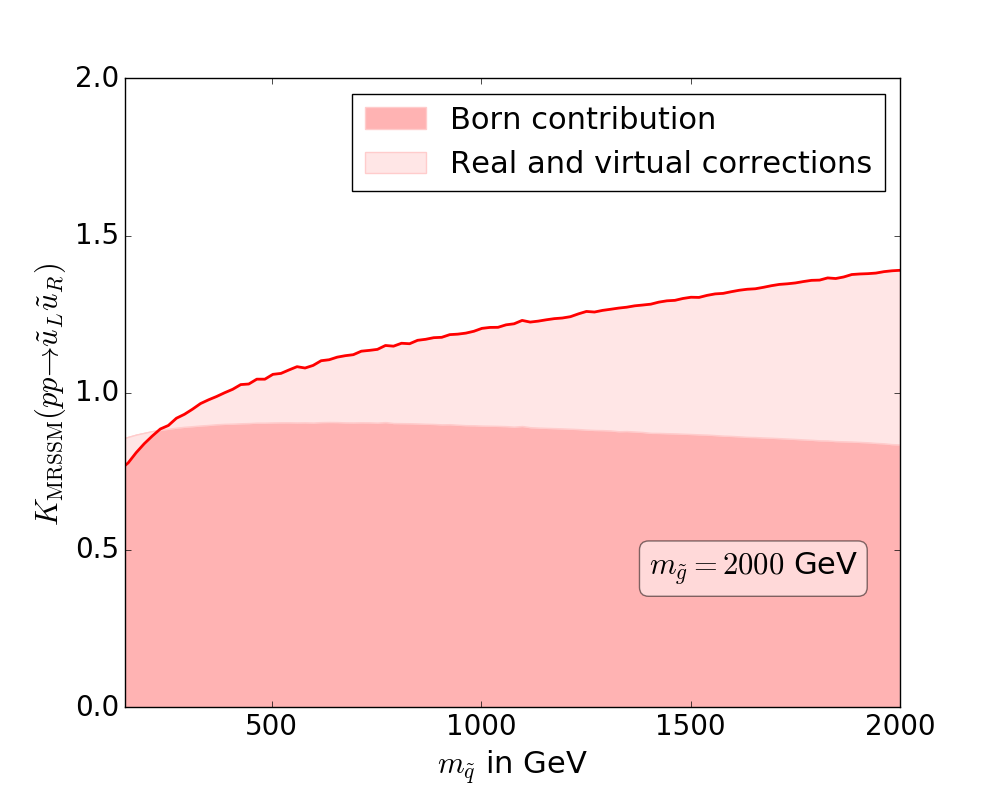
\includegraphics[scale=.4]{figures/MRSSM_uu_susu_Kfactors_msg=2000GeV.png}
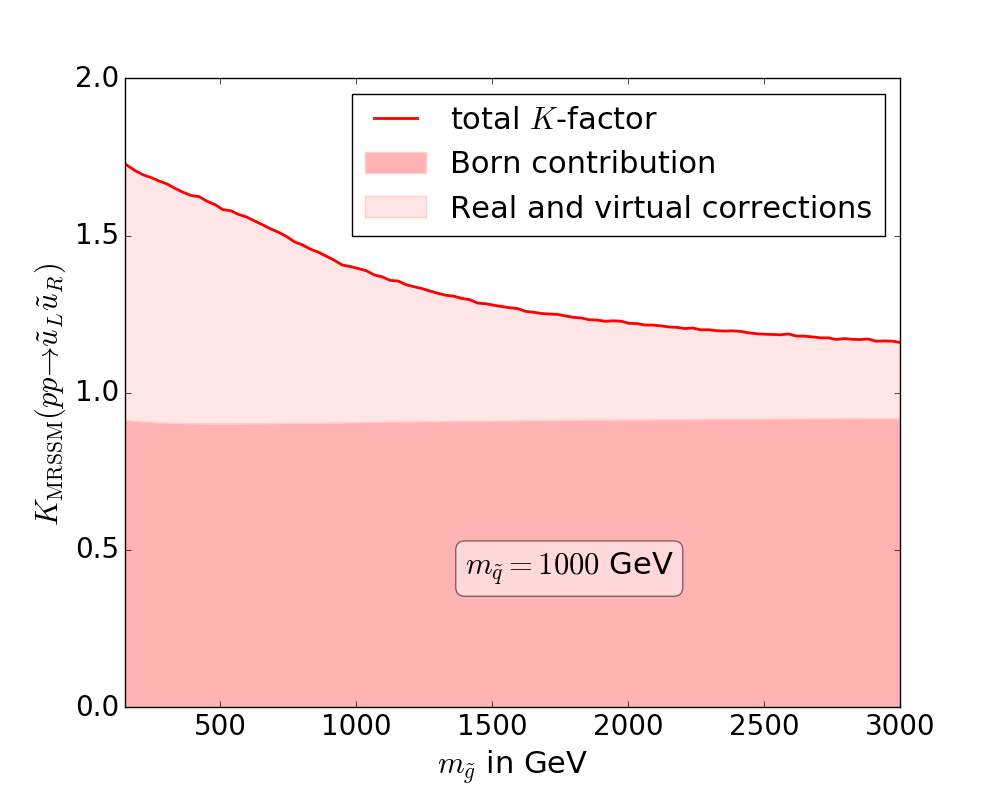
\includegraphics[scale=.4]{figures/MRSSM_uu_susu_Kfactors_msq=1000GeV.png}
\caption{Dependence of the $K$-factor for the process $uu \to \tilde{u}_L\tilde{u}_R$ in the MRSSM on the squark mass $m_{\tilde{q}}$ for fixed $m_{\tilde{g}} = \unit[2000]{GeV}$ (top) and on the gluino mass $m_{\tilde{g}}$ for fixed $m_{\tilde{q}} = \unit[1000]{GeV}$ (bottom). The other parameters are $\sqrt{S} = \unit[13]{TeV}$, $m_{\tilde{\sigma}} = \unit[5000]{GeV}$ and $\mu_R = \mu_F = m_{\tilde{q}}$. The used parton density function are the one from table \ref{tab:MRSSMKfactors}. The missing smoothness of the plot originates from the uncertainty of the integration.}\label{fig:1LXsection_fixed_m_MRSSM}
\end{center}
\end{figure}
Note further, that within the real corrections, only gluon radiation is included. This is because quark radiation, as described in section \ref{sec:RealQuarkRad}, involves the treatment of on-shell singularities which have unfortunately not been dealt with, due to a limited time budget. However, \cite{Gavin:2013kga} suggests that quark radiation gives only a sub percent effect to the next-to-leading order cross section of squark production when $m_{\tilde{g}} < m_{\tilde{q}}$. Of course, this argument applies to the MSSM but as the only difference to the MRSSM comes from diagrams involving gluinos and sgluons it provides also a strong argument for the suppression of quark radiation in the MRSSM. In fact, sgluons do not appear at all in diagrams contributing to real corrections. Furthermore, the change from Majorana to Dirac gluinos can never imply an amplification of processes involving gluinos. The reason for this is that if a gluino undergoes, due to its mass, a chirality flip, the right handed part of it, namely the octino, does neither couple to quarks nor to squarks. However, the effect of quark radiation is thought to increase when $m_{\tilde{g}} > m_{\tilde{q}}$. This is quantified within the next section, when squark production is discussed in the MSSM. Nonetheless, quark radiation is by no means to be thought of a dominant contribution to squark production at next-to-leading order.\\
Table \ref{tab:MRSSMKfactors} shows $\sigma^{\mathrm{LO}}$ and $\sigma^{\mathrm{NLO}}$ as they have been calculated by the devised \texttt{C++} program.
\begin{table}[H]
\begin{center}
\begin{tabular}{c|c?c|c|c}
$m_{\tilde{q}}$ in GeV & $m_{\tilde{g}}$ in GeV & $\sigma^{\mathrm{LO}}$ in fb & $\sigma^{\mathrm{NLO}}$ in fb & $K$\\
\hlinewd{2pt}
$500$ & $500$ & $966.4$ & $1440$ & $1.49$\\
$500$ & $1000$ & $303.4$ & $383$ & $1.26$\\
$1000$ & $1000$ & $42.63$ & $61.8$ & $1.45$\\
$1000$ & $2000$ & $11.56$ & $14.3$ & $1.24$\\
$1500$ & $3000$ & $0.9166$ & $1.13$ & $1.23$
\end{tabular}
\caption{$K$-factors of the process $pp \to \tilde{u}_L\tilde{u}_R$  in the MRSSM for a selected set of masses. The center-of-mass energy is $\sqrt{S} = \unit[13]{TeV}$ and the pseudoscalar mass is fixed to \mbox{$m_{\mathrm{\sigma}} = \unit[5000]{GeV}$}. For $\sigma^{\mathrm{LO}}$ parton density functions \texttt{MMHT2014}(LHAPDF ID: $25000$) has been used, whereas for $\sigma^{\mathrm{NLO}}$ \texttt{MMHT2014}(LHAPDF ID: $25100$) was used.}\label{tab:MRSSMKfactors}
\end{center}
\end{table}
It can be seen that the $K$-factors depend strongly on the ratio $\frac{m_{\tilde{g}}}{m_{\tilde{q}}}$ but not that strongly on the masses itself.\\
For three different choices of $m_{\tilde{q}}$ and $m_{\tilde{g}}$, Philip Dießner checked the results up to permille accuracy by doing the calculation using \texttt{GoSam}\cite{Cullen:2014yla, Cullen:2011ac} and \texttt{MadGraph5\_aMC@NLO}\cite{Alwall:2014hca} on the basis of the same model file.\\
The next-to-leading order cross sections of this chapter bear a relative uncertainty of one percent due to the numerical integration. The uncertainty which corresponds to the variation of the scales $\mu_R$ and $\mu_F$, see section \ref{sec:tree-level_cross_sections}, are evaluate to around 15\%.


\subsubsection{$K$-factors for Squark Production in the MSSM}
To compare the results of $K$-factors in the MRSSM to those in the MSSM, the cross sections in question have been calculated using the program \texttt{MadGraph5\_aMC@NLO} with the same parton density functions as before, i.e. \texttt{MMHT2014}. When generating the code for the pertaining processes, e.g. two protons to $\tilde{u}_L + \tilde{u}_R$, with
\begin{lstlisting}[style=Mybash]
generate p p > ul ur [QCD] $$go
\end{lstlisting}
the $s$-channel gluinos were omitted, with the addendum \texttt{\$\$go} as \texttt{MadGraph5} does not deal with divergences coming from the gluino in the on-shell limit. 
\begin{figure}[!htpb]
\begin{center}
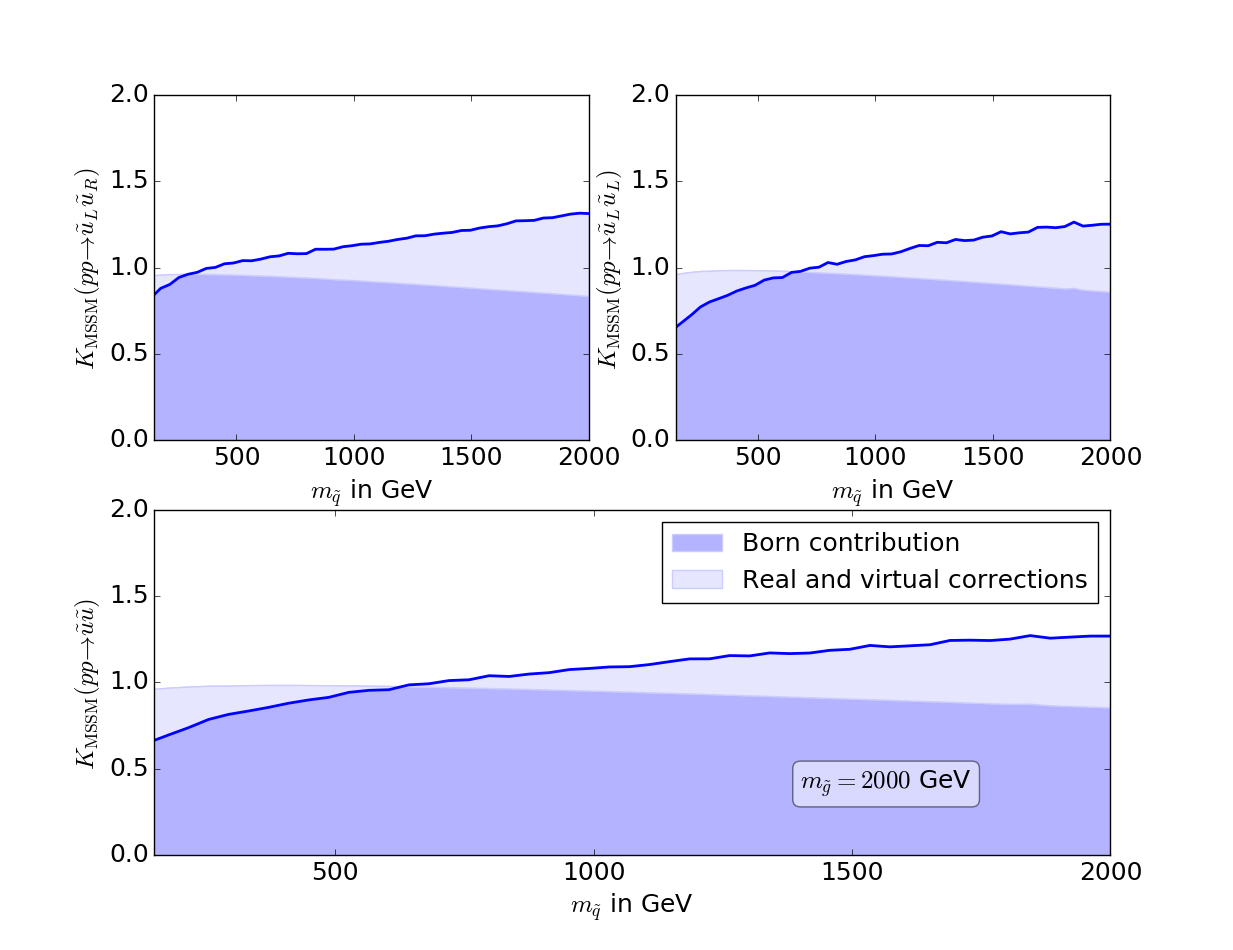
\includegraphics[scale=.47]{figures/MSSM_uu_susu_Kfactors_msg=2000GeV.png}
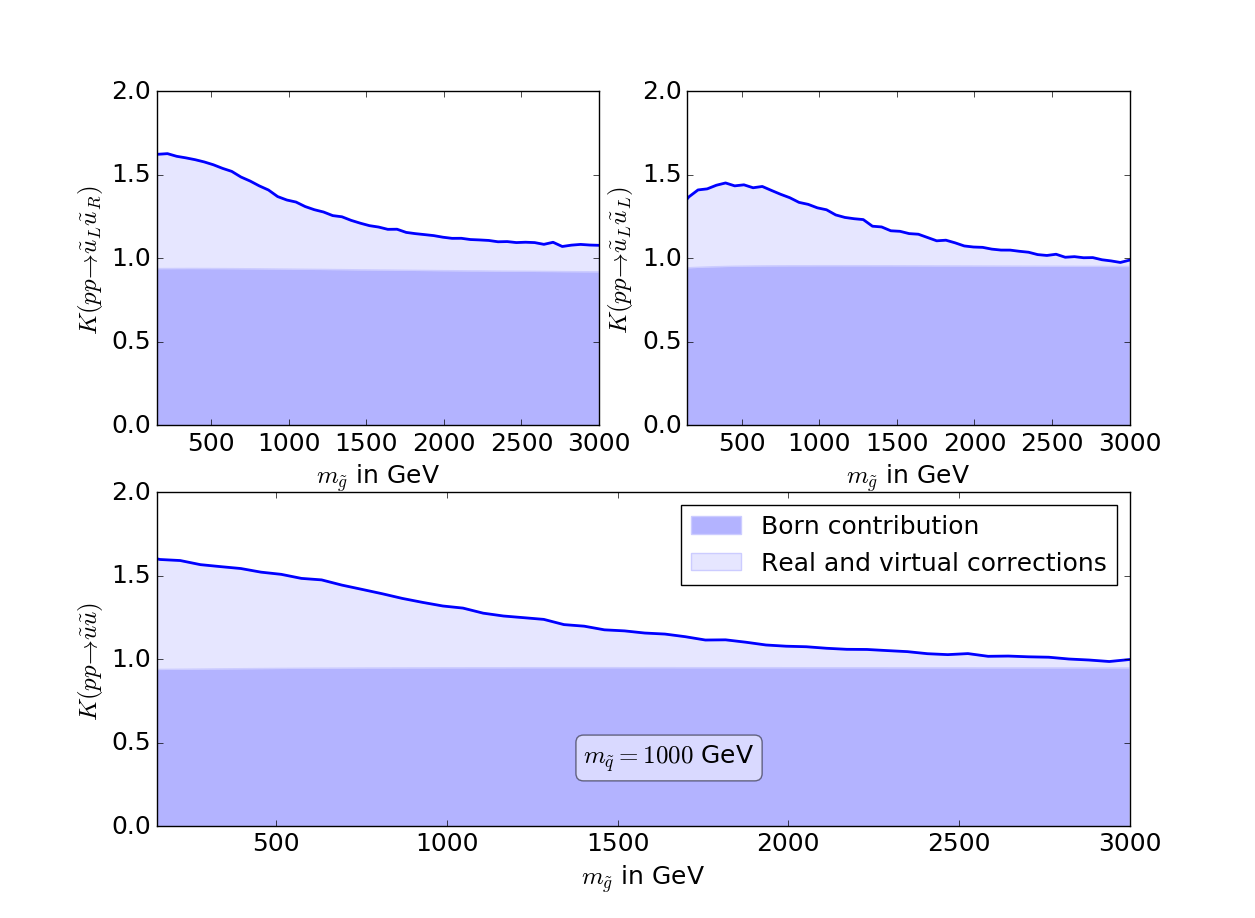
\includegraphics[scale=.47]{figures/MSSM_uu_susu_Kfactors_msq=1000GeV.png}
\caption{Dependence of the $K$-factor for the process $pp \to \tilde{u}\tilde{u}$, where $\tilde{u}\tilde{u} \in \left\{ \tilde{u}_L\tilde{u}_R, \tilde{u}_L\tilde{u}_L, \tilde{u}_R\tilde{u}_R \right\}$, in the MSSM on the squark mass $m_{\tilde{q}}$ for fixed $m_{\tilde{g}} = \unit[2000]{GeV}$ (top) and on the gluino mass $m_{\tilde{g}}$ for fixed $m_{\tilde{q}} = \unit[1000]{GeV}$ (bottom). The parameters are chosen like in fig. \ref{fig:1LXsection_fixed_m_MRSSM}.The $K$-factors have been broken down to contributions coming from $pp \to \tilde{u}_L\tilde{u}_R$ and from $pp \to \tilde{u}_L\tilde{u}_L$. The latter equals the contributions coming from $pp \to \tilde{u}_R\tilde{u}_R$. The missing smoothness of the plot originates from the uncertainty of the integration.}\label{fig:1LXsection_fixed_m_MSSM}
\end{center}
\end{figure}
As already discussed, these contributions are only of sub percent order when $m_{\tilde{q}} > m_{\tilde{g}}$\cite{Gavin:2013kga} but increase for $m_{\tilde{g}} > m_{\tilde{q}}$ as indicated in table \ref{tab:MSSMMadGraphProspino}, which compares $\sigma^{\mathrm{NLO}}$ obtained using \texttt{MadGraph5} and the program \texttt{Prospino2}\cite{Beenakker:1996ed} for both scenarios.

\begin{table}[H]
\begin{center}
\begin{tabular}{c|c?c?c}
$m_{\tilde{q}}$ in GeV & $m_{\tilde{g}}$ in GeV & $\sigma^{\mathrm{NLO}}_{\texttt{MadGraph}}$ in fb & $\sigma^{\mathrm{NLO}}_{\texttt{Prospino2}}$ in fb \\
\hlinewd{2pt}
$1500$ & $1000$ & $9.49 \pm 0.03$ & $9.48 \pm 0.09$ \\
$1000$ & $2000$ & $13.32 \pm 0.05$ & $13.89 \pm 0.11$ 
\end{tabular}
\caption{$\sigma^{\mathrm{NLO}}(pp \to \tilde{u}_L\tilde{u}_R)$ in the MSSM obtained from \texttt{MadGraph5} and \texttt{Prospino2} for a selected set of masses. The center-of-mass energy is $\sqrt{S} = \unit[13]{TeV}$. The stated uncertainties originate from the phase space integration. Within the \texttt{MadGraph5} calculation, the $s$-channel gluino diagrams have been discarded. This becomes relevant only when $m_{\tilde{g}} > m_{\tilde{q}}$.}\label{tab:MSSMMadGraphProspino}
\end{center}
\end{table}

In fact, comparing $\sigma^{\mathrm{NLO}}(pp \to \tilde{u}_L\tilde{u}_R)$ from \texttt{MadGraph5} with the one obtained by using \texttt{Prospino2}, which does include quark radiation, shows good agreement for the case $m_{\tilde{g}} < m_{\tilde{q}}$ but a small deviation for $m_{\tilde{g}} > m_{\tilde{q}}$. The given uncertainties are the uncertainties of the integration over the phase space and the chosen parameters are: $\mu_F = \mu_R = m_{\tilde{q}}$ and $\sqrt{S} = \unit[13]{TeV}$.\\
Figure \ref{fig:1LXsection_fixed_m_MSSM} shows the $K$-factors for squark production in the MSSM, broken down to $K$-factors for ``chirality'' like ($\tilde{u}_L \tilde{u}_L$) and unlike squarks ($\tilde{u}_L \tilde{u}_R$). It can be seen, that the mass dependence of $K(pp \to \tilde{u}_L \tilde{u}_R)$ in the MSSM is quite similar to the one in the MRSSM and that the MSSM $K$-factors are slightly smaller than in the MSSM. However, the $K$-factors for ``chirality'' like squarks are distinctly larger. The mass dependence of them is quite the same as for the  $pp \to \tilde{u}_L \tilde{u}_R$ channel. The only difference is a local maximum of the $K$-factor as a function of the gluino mass at $m_{\tilde{g}} \approx \unit[500]{GeV}$, where $m_{\tilde{q}} = \unit[1000]{GeV}$. Adding the cross sections for the three possible channels $\tilde{u}_L \tilde{u}_R$, $\tilde{u}_L \tilde{u}_L$ and $\tilde{u}_R \tilde{u}_R$ together one ends up with $K$-factors which have the very similar mass dependence as in the MRSSM but which can, depending on the chosen parameters, be significantly smaller.\\
Table \ref{tab:KfactorsMSSM} displays the leading order and next-to-leading order cross section of up-squark production in the MSSM. The total cross section for the production of all possible channels $\left\{ \tilde{u}_L\tilde{u}_R, \tilde{u}_L\tilde{u}_L, \tilde{u}_R\tilde{u}_R \right\}$ is broken down to the contribution, coming from the channel $\tilde{u}_L\tilde{u}_R$ whose tree-level cross section is the same as in the MRSSM.

\begin{table}[H]
\begin{center}
\begin{tabular}{c|c?c|c|c?c|c|c}
\multicolumn{2}{c?}{} & \multicolumn{3}{c?}{$p + p \to \tilde{u}_L + \tilde{u}_R$} & \multicolumn{3}{c}{$p + p \to \tilde{u} + \tilde{u}$} \\
\hlinewd{2pt}
$m_{\tilde{q}}$ in GeV & $m_{\tilde{g}}$ in GeV & $\sigma^{\mathrm{LO}}$ in fb & $\sigma^{\mathrm{NLO}}$ in fb & $K$ & $\sigma^{\mathrm{LO}}$ in fb & $\sigma^{\mathrm{NLO}}$ in fb & $K$\\
\hlinewd{2pt}
$500$ & $500$ & $966.4$ & $1328$ & $1.37$ & $2333$ & $3102$ \ignore{1328+2*887} & $1.33$\\
$500$ & $1000$ & $303.4$ & $352$ & $1.16$ & $1271$ & $1393$ \ignore{353 + 2*520} & $1.10$\\
$1000$ & $1000$ & $42.63$ & $58.5$ & $1.37$ & $122.2$ & $161.3$ \ignore{58.5+2*51.4} & $1.32$\\
$1000$ & $2000$ & $11.56$ & $13.3$ & $1.15$ & $66.36$ & $72.1$ \ignore{13.3+2*29.4} & $1.09$\\
$1500$ & $3000$ & $0.9166$ & $1.05$ & $1.14$ & $7.045$ & $7.57$\ignore{1.05+2*3.26} & $1.07$
\end{tabular}
\caption{$K$-factors of the process $pp \to \tilde{u}_L\tilde{u}_R$ and $pp \to \tilde{u}\tilde{u}$, where $\tilde{u}\tilde{u} \in \left\{ \tilde{u}_L\tilde{u}_R, \tilde{u}_L\tilde{u}_L, \tilde{u}_R\tilde{u}_R \right\}$, in the MSSM for a selected set of masses. The center-of-mass energy is $\sqrt{S} = \unit[13]{TeV}$.}\label{tab:KfactorsMSSM}
\end{center}
\end{table}

Again, it is clearly visible that the $K$-factors depend rather strongly on the ratio $\frac{m_{\mathrm{g}}}{m_{\mathrm{q}}}$ but not so much on the masses itself. Comparing with the results from the MRSSM in table \ref{tab:MRSSMKfactors}, one can state that the $K$-factors of the MRSSM are slightly larger. This might be the case, as there are additional degrees of freedom in the $R$-symmetric model, namely the octino which enters the gluino self-energy contributions (see second diagram from the right in \ref{fig:GluinoSE}) and sgluons which enter box diagrams (see lower right diagram in \ref{fig:1loopdiagrams}). The dependence on the sgluon mass is discussed within the next section.\\
The uncertainties of next-to-leading order cross sections, due to the phase space integration, within this section are of percent order. The uncertainty which corresponds to the scale variation does not increase 15\%.



\subsection{The Cross Section in the Limit of Large Sgluon Masses}
The cross section for squark production does not exist in the limit of an infinitely large sgluon mass, instead it was found that it diverges logarithmically:
\begin{align}
\lim_{m_{\sigma}\to\infty} \sigma(qq \to \tilde{q}\tilde{q}) \sim \ln \frac{m_{\sigma}^2}{\mu^2}.
\end{align}

\begin{figure}[H]
\begin{center}
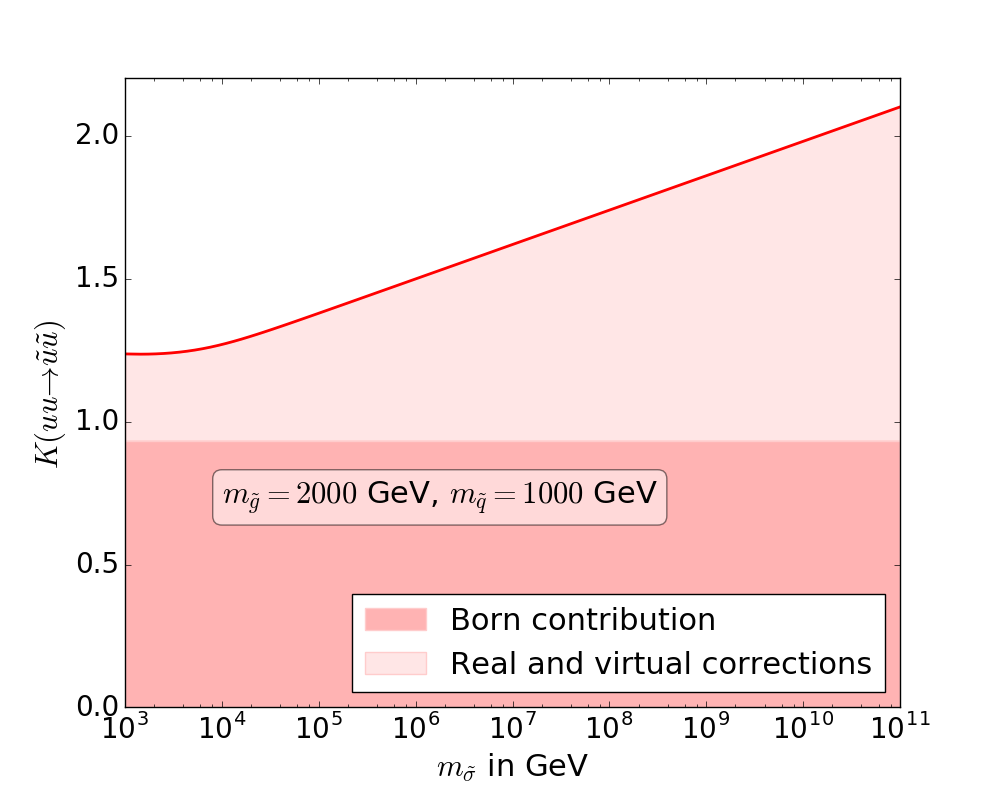
\includegraphics[scale=.5]{figures/MRSSM_uu_susu_Kfactors_msq=1000GeV_msg=2000GeV.png}
\caption{Dependence of the $K$-factor for the process $uu \to \tilde{u}\tilde{u}$ on the mass of the pseudoscalar sgluon. For $m_{\sigma} \approx \unit[10^5]{GeV}$ onwards want find a logarithmic scaling as predicted by \cite{Cheng:1997sq}.}\label{fig:SgluonMassDependence}
\end{center}
\end{figure}
This is actually expected as an effective field theory of the MRSSM where the sgluon is integrated out is no longer supersymmetric. This is because the sgluon is together with the octino part of a supermultiplet. Integrating out only the sgluon means that the octino misses its superpartner in the effective field theory. In this case the decoupling theorem \cite{Appelquist:1974tg} does no longer hold\footnote{It is even possible to predict the  logarithmic scaling of $\sigma(qq \to \tilde{q}\tilde{q})$ quantitatively. The coefficient of the logarithm is proportional to the difference of the one-loop $\beta$ function coefficients of $g_s$ and $\hat{g}_s$ in the effective theory with the heavy particle integrated out, see eq. (4) in \cite{Cheng:1997sq}.}.
The logarithmic scaling of the cross section as a function of the mass of the pseudoscalar is shown in fig. \ref{fig:SgluonMassDependence}.

